\subsubsection{Conditions}\label{sec:mapping-conditions}
\lstset{language=XML,numbers=left,xleftmargin=2em}

In \cite{MTCPart2}, the \mtmodel{DataItem} represents the metadata describing the semantic meaning of the \gls{MTCondition} as it relates to its component using an object instance of type \mtuatype{MTConditionType}. The activation and state of \glspl{MTCondition} is represented by the \mtuatype{MTConditionEventType} that is a subtype of the \uamodel{BaseConditionType}. The MTConnect \glspl{MTCondition} in \cite{MTCPart3} is a representation of the state of various alarms and health of a \gls{MTComponent} of the machine. There are three states for a condition in MTConnect, they are \mtmodel{Normal}, \mtmodel{Warning}, and \mtmodel{Fault} and have the semantic meaning \textit{operating normally}, \textit{a situation has been observed, but may self-correct}, and \textit{a failure has occured and needs manual intervention} respectively. More information can be found in MTConnect \cite{MTCPart2} and \cite{MTCPart3} of the MTConnect Standard for Condition modeling and behavior.

When a \gls{MTCondition} becomes active in MTConnect, it will transition from \mtmodel{Normal} to \mtmodel{Warning} or \mtmodel{Fault} state. The transition will cause an \uamodel{Event} to be dispatched of the \mtuatype{MTConditionEventType}. The \mtuatype{MTConditionEventType} has a \gls{Property} called \uamodel{ActiveState} that indicates that it is currently active. The \uamodel{ActiveState} is an OPC UA \uamodel{TwoStateVariableType} \uamodel{Variable} defined in \cite{UAPart8}. When a Condition is \mtmodel{Normal}, the \uamodel{ActiveState} is \uamodel{False}, otherwise when either a \mtmodel{Warning} or \mtmodel{Fault} is present, the \uamodel{ActiveState} is \uamodel{True}. An active \gls{MTCondition} will require the \uamodel{Retain} flag of the \mtuamodel{MTConditionEventType} instance to be \uamodel{True}.

\begin{lstlisting}[firstnumber=last,escapechar=|,%
    caption={Rotary C Component Stream},label={lst:rotary-component-stream}]
<ComponentStream componentId="zf476090" component="Rotary" name="C" nativeName="S">
  <Condition>
    <Normal sequence="201" timestamp="2018-10-31T20:34:19.9981Z" dataItemId="afb596b0" type="AMPERAGE" compositionId="b7792870" name="Soverload"/> |\label{line:amp-201}|
    <Warning sequence="503" timestamp="2018-10-31T20:45:19.9981Z" dataItemId="afb596b0" type="AMPERAGE" compositionId="b7792870" name="Soverload" qualifier="HIGH" nativeCode="MOT-WARN">Spindle Motor Warning</Warning> |\label{line:amp-503}|
    <Fault sequence="652" timestamp="2018-10-31T20:49:19.9981Z" dataItemId="afb596b0" type="AMPERAGE" compositionId="b7792870" name="Soverload" qualifier="HIGH" nativeCode="MOT-OVR">Spindle Motor Overload</Fault> |\label{line:amp-652}|
  </Condition>
  ...
\end{lstlisting} %

Each time an MTConnect \gls{MTCondition} activates or deactivates, a \gls{Condition} \gls{Event} will be reported associated with the meta-data instance of the \mtuatype{MTConditionType} using the \gls{NodeId} as the \uamodel{SourceNode} of the \uamodel{Event}.  \mtuatype{MTConditionEventType} is a subtype of the \gls{Event} and MUST never be instantiated in the address space as an \gls{Object}.

\paragraph{Mapping Conditions}

MTConnect allows \mtmodel{Conditions} to represent multiple instances simultaneous \mtterm{Faults} and \mtterm{Warnings} associated with a \mtmodel{Component} and of a particular \mtterm{Type}. In MTConnect a \mtterm{Type} can be something like a \mtmodel{TEMPERATURE} or a \mtmodel{LOGICAL_PROGRAM}. The \mtmodel{Conditions} \mtterm{Faults} and \mtterm{Warnings} are associated by their unique characteristics of their description or more commonly their \mtmodel{nativeCode}.

Every time a condition is reported as a separate instance, as described in \cite{MTCPart3}, it is consider another activation of the \mtterm{Condition} and will be associated with a unique \uamodel{ConditionId} as the specific \gls{NodeId} of the \mtuatype{MTConditionEventType}. The \uamodel{ConditionName} is handled in the same manner as the \uamodel{ConditionId} and must be unique for a stream of associated \mtterm{Condition} set of states. Only when a \mtmodel{Normal} with no \xml{nativeCode} cleared all active Conditions, or each are cleared separately (going back to a \mtmodel{Normal} state), does the condition report \mtmodel{Normal} when for a \mtmodel{current} request. When all active \mtterm{Condition} are have reported \mtmodel{Normal}, an \mtuatype{MTConditionEventType} for each active \mtterm{Condition} must be reported with the \mtmodel{ActiveState} set to \uamodel{False} and the \uamodel{Retain} set to \uamodel{False}.

The \gls{ConditionType} and \uamodel{EventType} properties will be set as follows:

\begin{table}[ht]
  \centering 
  \caption{Mapping to \texttt{MTConditionEventType} Properties  }
  \label{table:ua-condition-event-mapping}
  \fontsize{9pt}{11pt}\selectfont
  \tabulinesep=3pt
  \begin{tabu} to 6.5in {|l|l|X|} \everyrow{\hline}
    \hline
    \rowfont\bfseries {Property} & {Type} & {Mapping} \\
    \tabucline[1.5pt]{}
    (Attribute) NodeId & NodeId & A \uamodel{NodeId} associated with the MTConnect \mtterm{Condition} stream. Often given by
                                  the \mtmodel{nativeCode} attribute. Referred to as the \uamodel{ConditionId} \\
    EventId & ByteString & Auto-generated by the server per \cite{UAPart5} \\
    EventType & NodeId & The \uamodel{NodeId} of the \mtuatype{MTConditionEventType}. \\
    SourceNode & NodeId & The \uamodel{NodeId} of the \uaterm{Instance} of the \mtuatype{MTConditionType} \uaterm{Object}
                          representing the \mtmodel{DataItem} with \mtmodel{category} \mtmodel{CONDITION}. \\
    SourceName & NodeId & The \uamodel{BrowseName} of the \uamodel{SourceNode} referenced above. \\
    Time & UtcTime & From MTConnect timestamp attribute. \\
    ReceiveTime & UtcTime & Current time when MTConnect Condition received by OPC UA Server. \\
    LocalTime & TimeZoneDataType & Optionally supplied by OPC UA Server since MTConnect uses UTC. \\
    Message & LocalizedText & MTConnect Condition \texttt{CDATA}. \\
    Severity & UInt16 &
    Taking the value for the \mtterm{QName} of the \mtmodel{Condition}:
    \begin{itemize}
      \setlength\itemsep{0em}
      \item When \mtmodel{Normal}, \uamodel{Severity} is 0.
      \item When \mtmodel{Warning}, \uamodel{Severity} is 500.
      \item When \mtmodel{Fault}, \uamodel{Severity} is 1000.
    \end{itemize} \\
    ConditionClassId & NodeId & The \uamodel{NodeId} for the \mtmodel{ClassType} representing the \mtmodel{type}
                                 attribute of the \mtmodel{DataItem}. \\
    ConditionClassName & LocalizedText & The name associated with the \uamodel{ConditionClassId}. \\
    ConditionSubClassId & NodeId & The \uamodel{NodeId} for the \mtmodel{ClassType} representing the \mtmodel{subType}
                                 attribute of the \mtmodel{DataItem}. \\
    ConditionSubClassName & LocalizedText & The name associated with the \uamodel{ConditionSubClassId}. \\
    ConditionName & String & A text version of the set of associated conditions, should follow the same rules as the \uamodel{ConditionId}. For example, the name MAY be composed of the \mtmodel{SourceName} and the \mtmodel{nativeCode}. \\
    BranchId & NodeId & Not used for MTConnect. \\
    Retain & Boolean &
    Taking the value for the \mtterm{QName} of the \mtmodel{Condition}:
    \begin{itemize}
      \setlength\itemsep{0em}
      \item When only \mtmodel{Normal}, \uamodel{False}
      \item When \mtmodel{Warning} or \mtmodel{Fault}, \uamodel{True}
    \end{itemize} \\
    EnabledState & LocalizedText &
    Taking the value for the \mtterm{QName} of the \mtmodel{Condition}:
    \begin{itemize}
      \setlength\itemsep{0em}
      \item When \mtmodel{Unavailable}, \uamodel{Disabled}
      \item Otherwise, \uamodel{Enabled}
    \end{itemize}  \\
    Quality & StausCode & 
    Taking the value for the \mtterm{QName} of the \mtmodel{Condition}:
    \begin{itemize}
      \setlength\itemsep{0em}
      \item When \mtmodel{Unavailable}, \uamodel{Bad_NotConnected}
      \item Otherwise, \uamodel{Good}
    \end{itemize}  \\
    LastSeverity & Uint16 & Set to the previous severity for this condition. \\
    Comment & LocalizedText & Set to the \mtterm{CDATA} of the Condition. \\
    ClientUserId & String & The \mtmodel{name} of the \mtmodel{Device}. \\
    ActiveState & LocalizedText &
    Taking the value for the \mtterm{QName} of the \mtmodel{Condition}:
    \begin{itemize}
      \setlength\itemsep{0em}
      \item When only \mtmodel{Normal}, \uamodel{Inactive}
      \item When \mtmodel{Warning} or \mtmodel{Fault}, \uamodel{Active}
    \end{itemize} \\
  \end{tabu}
\end{table}

\FloatBarrier

\paragraph{MTConnect Condition Parallel Activation}

As stated above, MTConnect allows for multiple \mtmodel{Condition}s of the same type to be active at the same time. In MTConnect the conditions can be differentiated by their \mtmodel{nativeCode} or \gls{CDATA}. In the following example, the attribute \mtmodel{nativeCode} is used to indicate the independent activations of the \mtmodel{Condition}. In this diagram, there are three activation--0, 1, and 2--of the PLC alarms and are associated with the \mtmodel{LOGIC_PROGRAM}. Each of the unique \mtmodel{nativeCode}s is mapped an \uamodel{Event}  and tracked separately. 

The \mtmodel{Condition} is instantiated in the \uamodel{AddressSpace} as an \mtuatype{MTConditionType} and acts as the source of the \uamodel{Event}s when they are sent. The individual activation and deactivations are tracked using the \uamodel{Event} mechanism as described in \cite{UAPart3} and \cite{UAPart4}. All \uamodel{Event}s will have the same \uamodel{SourceNode} since they are all produced from the same \mtuatype{MTConditionType} instance.

Table~\ref{table:ua-condition-states} represents the state transitions of the key OPC UA \uamodel{Condition} model and the reporting of \mtuatype{MTConditionEventType}. The text that follows will refer to this table and the MTConnect \gls{xml} to illustrate the expected behavior. Figure~\ref{fig:condition-branching} gives a visual representation of the event reporting.

\begin{table}[ht]
  \centering 
  \caption{\texttt{LogicProgramCondition} States}
  \label{table:ua-condition-states}
  \fontsize{9pt}{11pt}\selectfont
  \tabulinesep=3pt
  \newcounter{condrownumbers}
  \newcommand\rownumber{\stepcounter{condrownumbers}\arabic{condrownumbers}}
  \begin{tabu} to 6in {|X[0.25,r]|X|X|X|X[3]|} \everyrow{\hline}
    \hline
    \rowfont\bfseries {Seq} & {Active} & {Retain} & {Native Code} & {Message} \\
    \tabucline[1.5pt]{}
    \rownumber & false & false & NULL & NULL \\
    \rownumber & true & true & PLC--154 & PIN SENSOR MALF \\
    \rownumber & true & true & PLC--155 & WORK NO. ERROR(0 OR >9999) \\
    \rownumber & true & true & PLC--157 & WARMING UP!!! \\
    \rownumber & false & false & PLC--154 & PIN SENSOR MALF \\
    \rownumber & false & false & PLC--157 & WARMING UP!!! \\
    \rownumber & false & false & PLC--155 & WORK NO. ERROR(0 OR >9999) \\
    \rownumber & false & false & NULL & NULL \\
  \end{tabu}
\end{table}

\begin{figure}[ht]
  \centering
  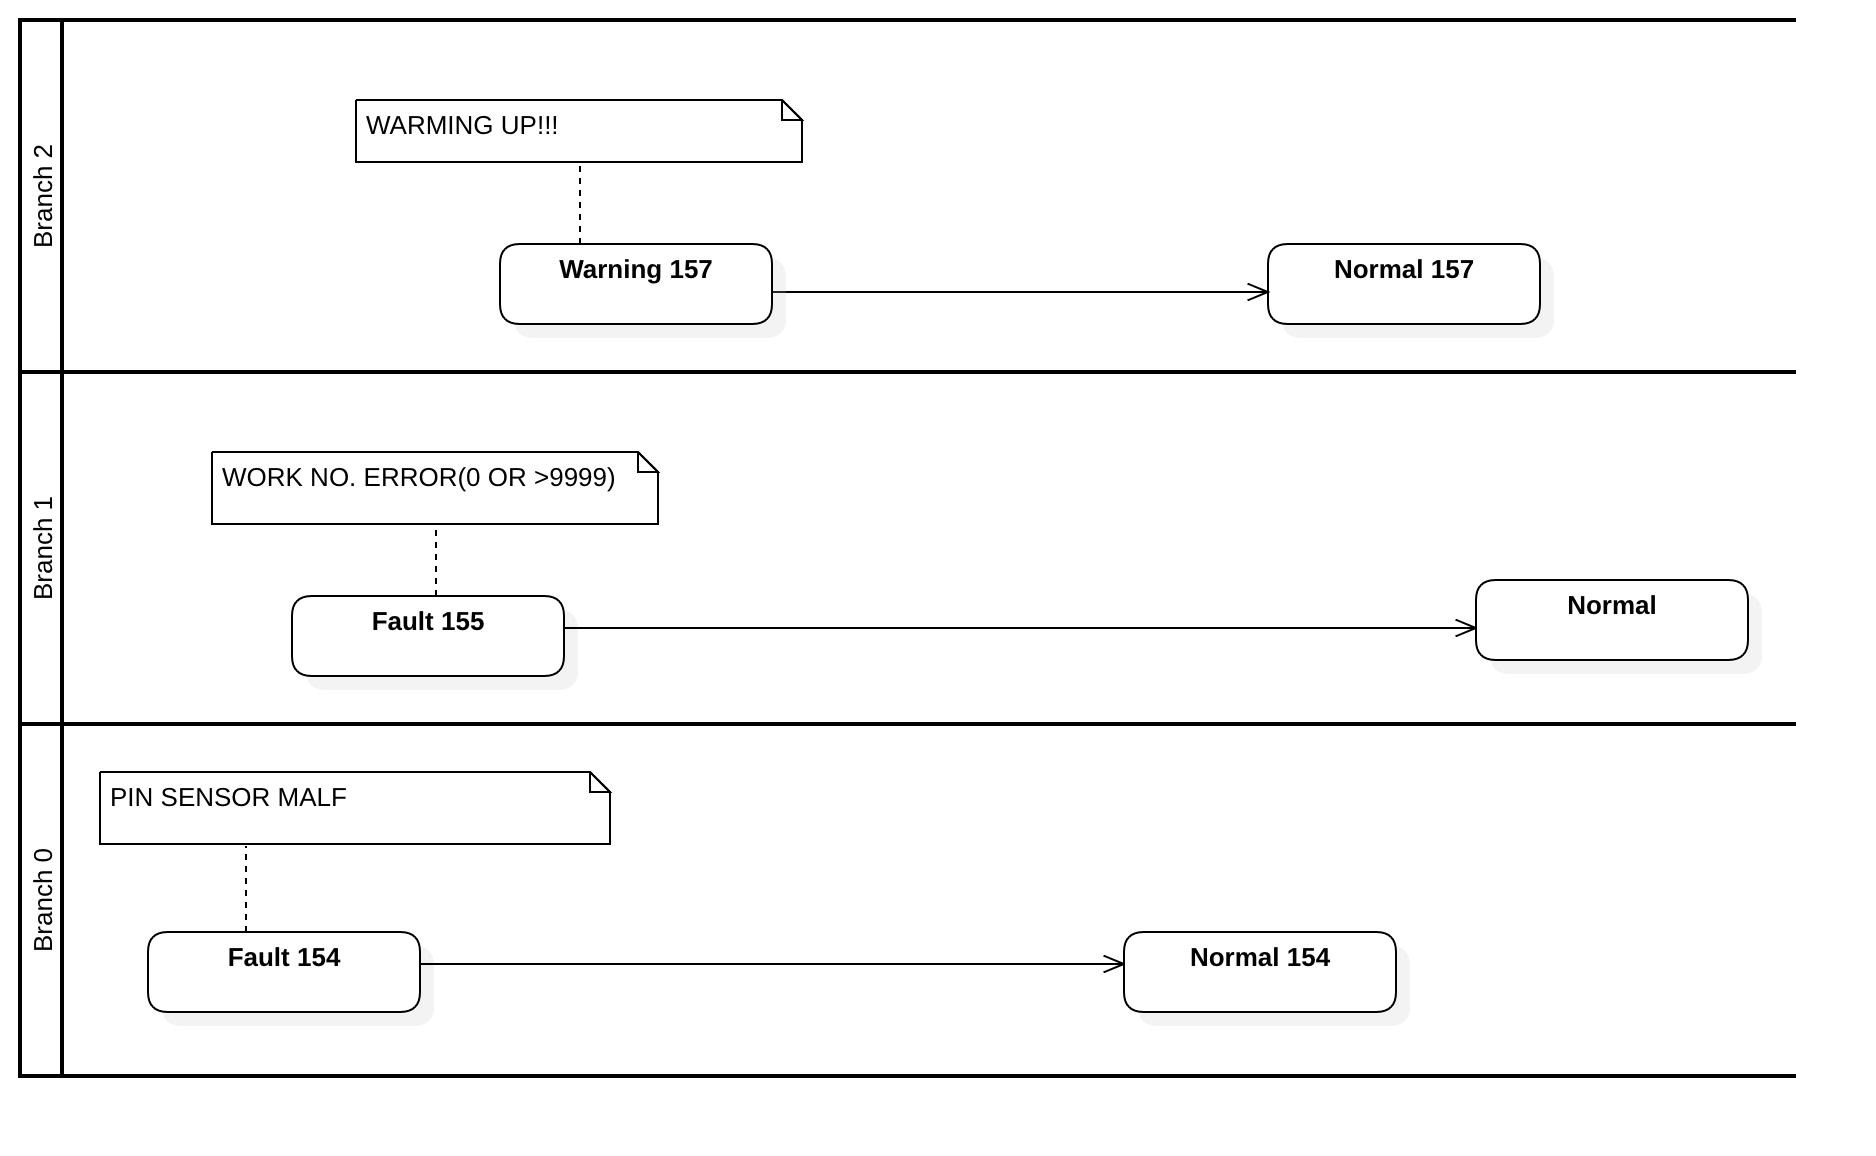
\includegraphics[width=1.0\textwidth]{diagrams/mtconnect-mapping/condition-branching.png}
  \caption{Parallel Conditions}
  \label{fig:condition-branching}
\end{figure}

For this example, MTConnect uses the \mtmodel{nativeCode} to determine the uniqueness of each activation of the Condition. If the \mtterm{Path} component has a \gls{MTDataItem} with a \gls{type} of \mtmodel{LOGIC_PROGRAM} and given in listing~\ref{lst:controller-component}, the \gls{MTDataItem} will be represented in the OPC UA model as a instance of the \mtuatype{MTConditionType} with the attributes presented as properties.

The initial state of the system is given in Table~\ref{table:ua-condition-states} Row~1. When the condition is inactive, the \uamodel{AciveState} property is \uamodel{false} and the \uamodel{Retain} flag is also set to \uamodel{false}. This corresponds to Listing~\ref{lst:path-logic-program-condition-0} and the \mtmodel{Normal} initial condition state with no \mtmodel{nativeCode} indicating there are no active conditions.

\begin{lstlisting}[firstnumber=1,escapechar=|,%
    caption={Path Logic Program Initial Normal State},label={lst:path-logic-program-condition-0}]
  <ComponentStream componentId="a4a7bdf0" component="Path" name="P1">
    <Condition>
      <Normal sequence="5200" timestamp="2018-10-31T20:30:19.9981Z" dataItemId="a557d330" type="LOGIC_PROGRAM"/>
    </Condition>
  </ComponentStream>
\end{lstlisting}

The first fault occurred with the \mtmodel{nativeCode} \mtmodel{PLC-154} and reports an \uamodel{Event} \mtuatype{MTConditionEventType} as shown in Listing~\ref{lst:path-logic-program-condition-1}. A \mtmodel{Fault} indicates a situation where the piece of equipment is no longer able to continue functioning and needs manual intervention.

\begin{lstlisting}[firstnumber=last,escapechar=|,%
    caption={Path Logic Program First Fault PLC-154},label={lst:path-logic-program-condition-1}]
  <ComponentStream componentId="a4a7bdf0" component="Path" name="P1">
    <Condition>
      <Fault sequence="5201" timestamp="2018-10-31T20:34:19.9981Z" dataItemId="a557d330" type="LOGIC_PROGRAM" nativeCode="PLC-154">PIN SENSOR MALF</Fault>
    </Condition>
  </ComponentStream>
\end{lstlisting}

The second \mtmodel{Fault} is given in Listing~\ref{lst:path-logic-program-condition-2} where a second PLC alarm is active. The native code is different than the previous condition, so a second \mtuatype{MTConditionEventType} must be reported with a unique \uamodel{ConditionId} indicated using the \uamodel{NodeId} in the \uamodel{Event}. 

\begin{lstlisting}[firstnumber=last,escapechar=|,%
    caption={Path Logic Program Second Fault PLC-155},label={lst:path-logic-program-condition-2}]
  <ComponentStream componentId="a4a7bdf0" component="Path" name="P1">
    <Condition>
      <Fault sequence="5209" timestamp="2018-10-31T20:36:19.9981Z" dataItemId="a557d330" type="LOGIC_PROGRAM" nativeCode="PLC-155">WORK NO. ERROR(0 OR >9999)</Fault>
    </Condition>
  </ComponentStream>
\end{lstlisting}

The warning in Listing~\ref{lst:path-logic-program-condition-3} indicates the machine is warming up and other operations are disabled. This condition has another \mtmodel{nativeCode} and therefor, like the previous condition, another \uamodel{Event} must sentreported. The \mtmodel{Warning} will be represented in UA as a \uamodel{severity} and represents something that is of concern but not stopping the process. The warning is given by Row~4 of Table~\ref{table:ua-condition-states}.

\begin{lstlisting}[firstnumber=last,escapechar=|,%
    caption={Path Logic Program Warning PLC-157},label={lst:path-logic-program-condition-3}]
  <ComponentStream componentId="a4a7bdf0" component="Path" name="P1">
    <Condition>
      <Warning sequence="5318" timestamp="2018-10-31T20:42:19.9981Z" dataItemId="a557d330" type="LOGIC_PROGRAM" nativeCode="PLC-157">WARMING UP!!!</Warning>
    </Condition>
  </ComponentStream>
\end{lstlisting}

In Listing~\ref{lst:path-logic-program-condition-4}, when the sensor malfunction is reset, the first condition will be returned to an inactive state. This is indicated by \mtmodel{Normal} and a native code of \mtmodel{PLC-154}. Since the other two conditions are still active. In MTConnect, a \mtmodel{current} request would indicate that there is a Fault and a Warning currently active for this \mtmodel{Condition}. The clearing of this individual \mtmodel{Fault} is also represented on Row~5 of Table~\ref{table:ua-condition-states}. An \mtuatype{MTConditionEventType} \uamodel{Event} will be reported with its \mtmodel{ActiveState} set to \uamodel{False} and \uamodel{Retain} property set to \uamodel{False}.

\begin{lstlisting}[firstnumber=last,escapechar=|,%
    caption={Path Logic Program Clear Fault of PLC-154},label={lst:path-logic-program-condition-4}]
  <ComponentStream componentId="a4a7bdf0" component="Path" name="P1">
    <Condition>
      <Normal sequence="5467" timestamp="2018-10-31T20:51:19.9981Z" dataItemId="a557d330" type="LOGIC_PROGRAM" nativeCode="PLC-154"/>
    </Condition>
  </ComponentStream>
\end{lstlisting}

In Listing~\ref{lst:path-logic-program-condition-5}, when the machine finishes warming up, the first condition will be returned to an inactive state. It is indicated by \mtmodel{Normal} and a native code of \mtmodel{PLC-157} and will be handled like the previous case. In MTConnect, a \mtmodel{current} request would indicate that there is a Fault and a Warning currently active for this \mtmodel{Condition}. Similar to the previous state, Table~\ref{table:ua-condition-states} clears the active state of this \uamodel{Event} on Row~6.

\begin{lstlisting}[firstnumber=last,escapechar=|,%
    caption={Path Logic Program Clear Warning PLC-157},label={lst:path-logic-program-condition-5}]
  <ComponentStream componentId="a4a7bdf0" component="Path" name="P1">
    <Condition>
      <Normal sequence="5467" timestamp="2018-10-31T20:52:19.9981Z" dataItemId="a557d330" type="LOGIC_PROGRAM" nativeCode="PLC-157"/>
    </Condition>
  </ComponentStream>
\end{lstlisting}

Listing~\ref{lst:path-logic-program-condition-6} represents the final \mtmodel{Normal} transition that clears all the currently active conditions and indicates that all the \mtmodel{Conditions} are now inactive or cleared and back to a \mtmodel{Normal} state. Row~7 of Table~\ref{table:ua-condition-states} shows the clearing of the final activation and then we clear everything in Row~8.

\begin{lstlisting}[firstnumber=last,escapechar=|,%
    caption={Path Logic Program Back to Normal, All Clear},label={lst:path-logic-program-condition-6}]
  <ComponentStream componentId="a4a7bdf0" component="Path" name="P1">
    <Condition>
      <Normal sequence="5467" timestamp="2018-10-31T20:57:19.9981Z" dataItemId="a557d330" type="LOGIC_PROGRAM"/>
    </Condition>
  </ComponentStream>
\end{lstlisting}


%%% Local Variables:
%%% mode: latex
%%% TeX-master: "main"
%%% End:
